%The importance of hardware parameters on packet processing is not well understood.
%We study the impact of low-end hardware on packet processing.
%We use iPerf tool to measure the network throughput under controlled conditions. We host an ad hoc WiFi network using Aruba WiFi AP in an interference free environment with a link speed of 72Mbps.
%We use a Linux laptop as server and Nexus4 mobile phone as a client.
%We vary the CPU clock frequency and load parameters to measure both file download time and throughput

\begin{figure}[t!]
     \subfloat[Download Time vs. Clock]{%
       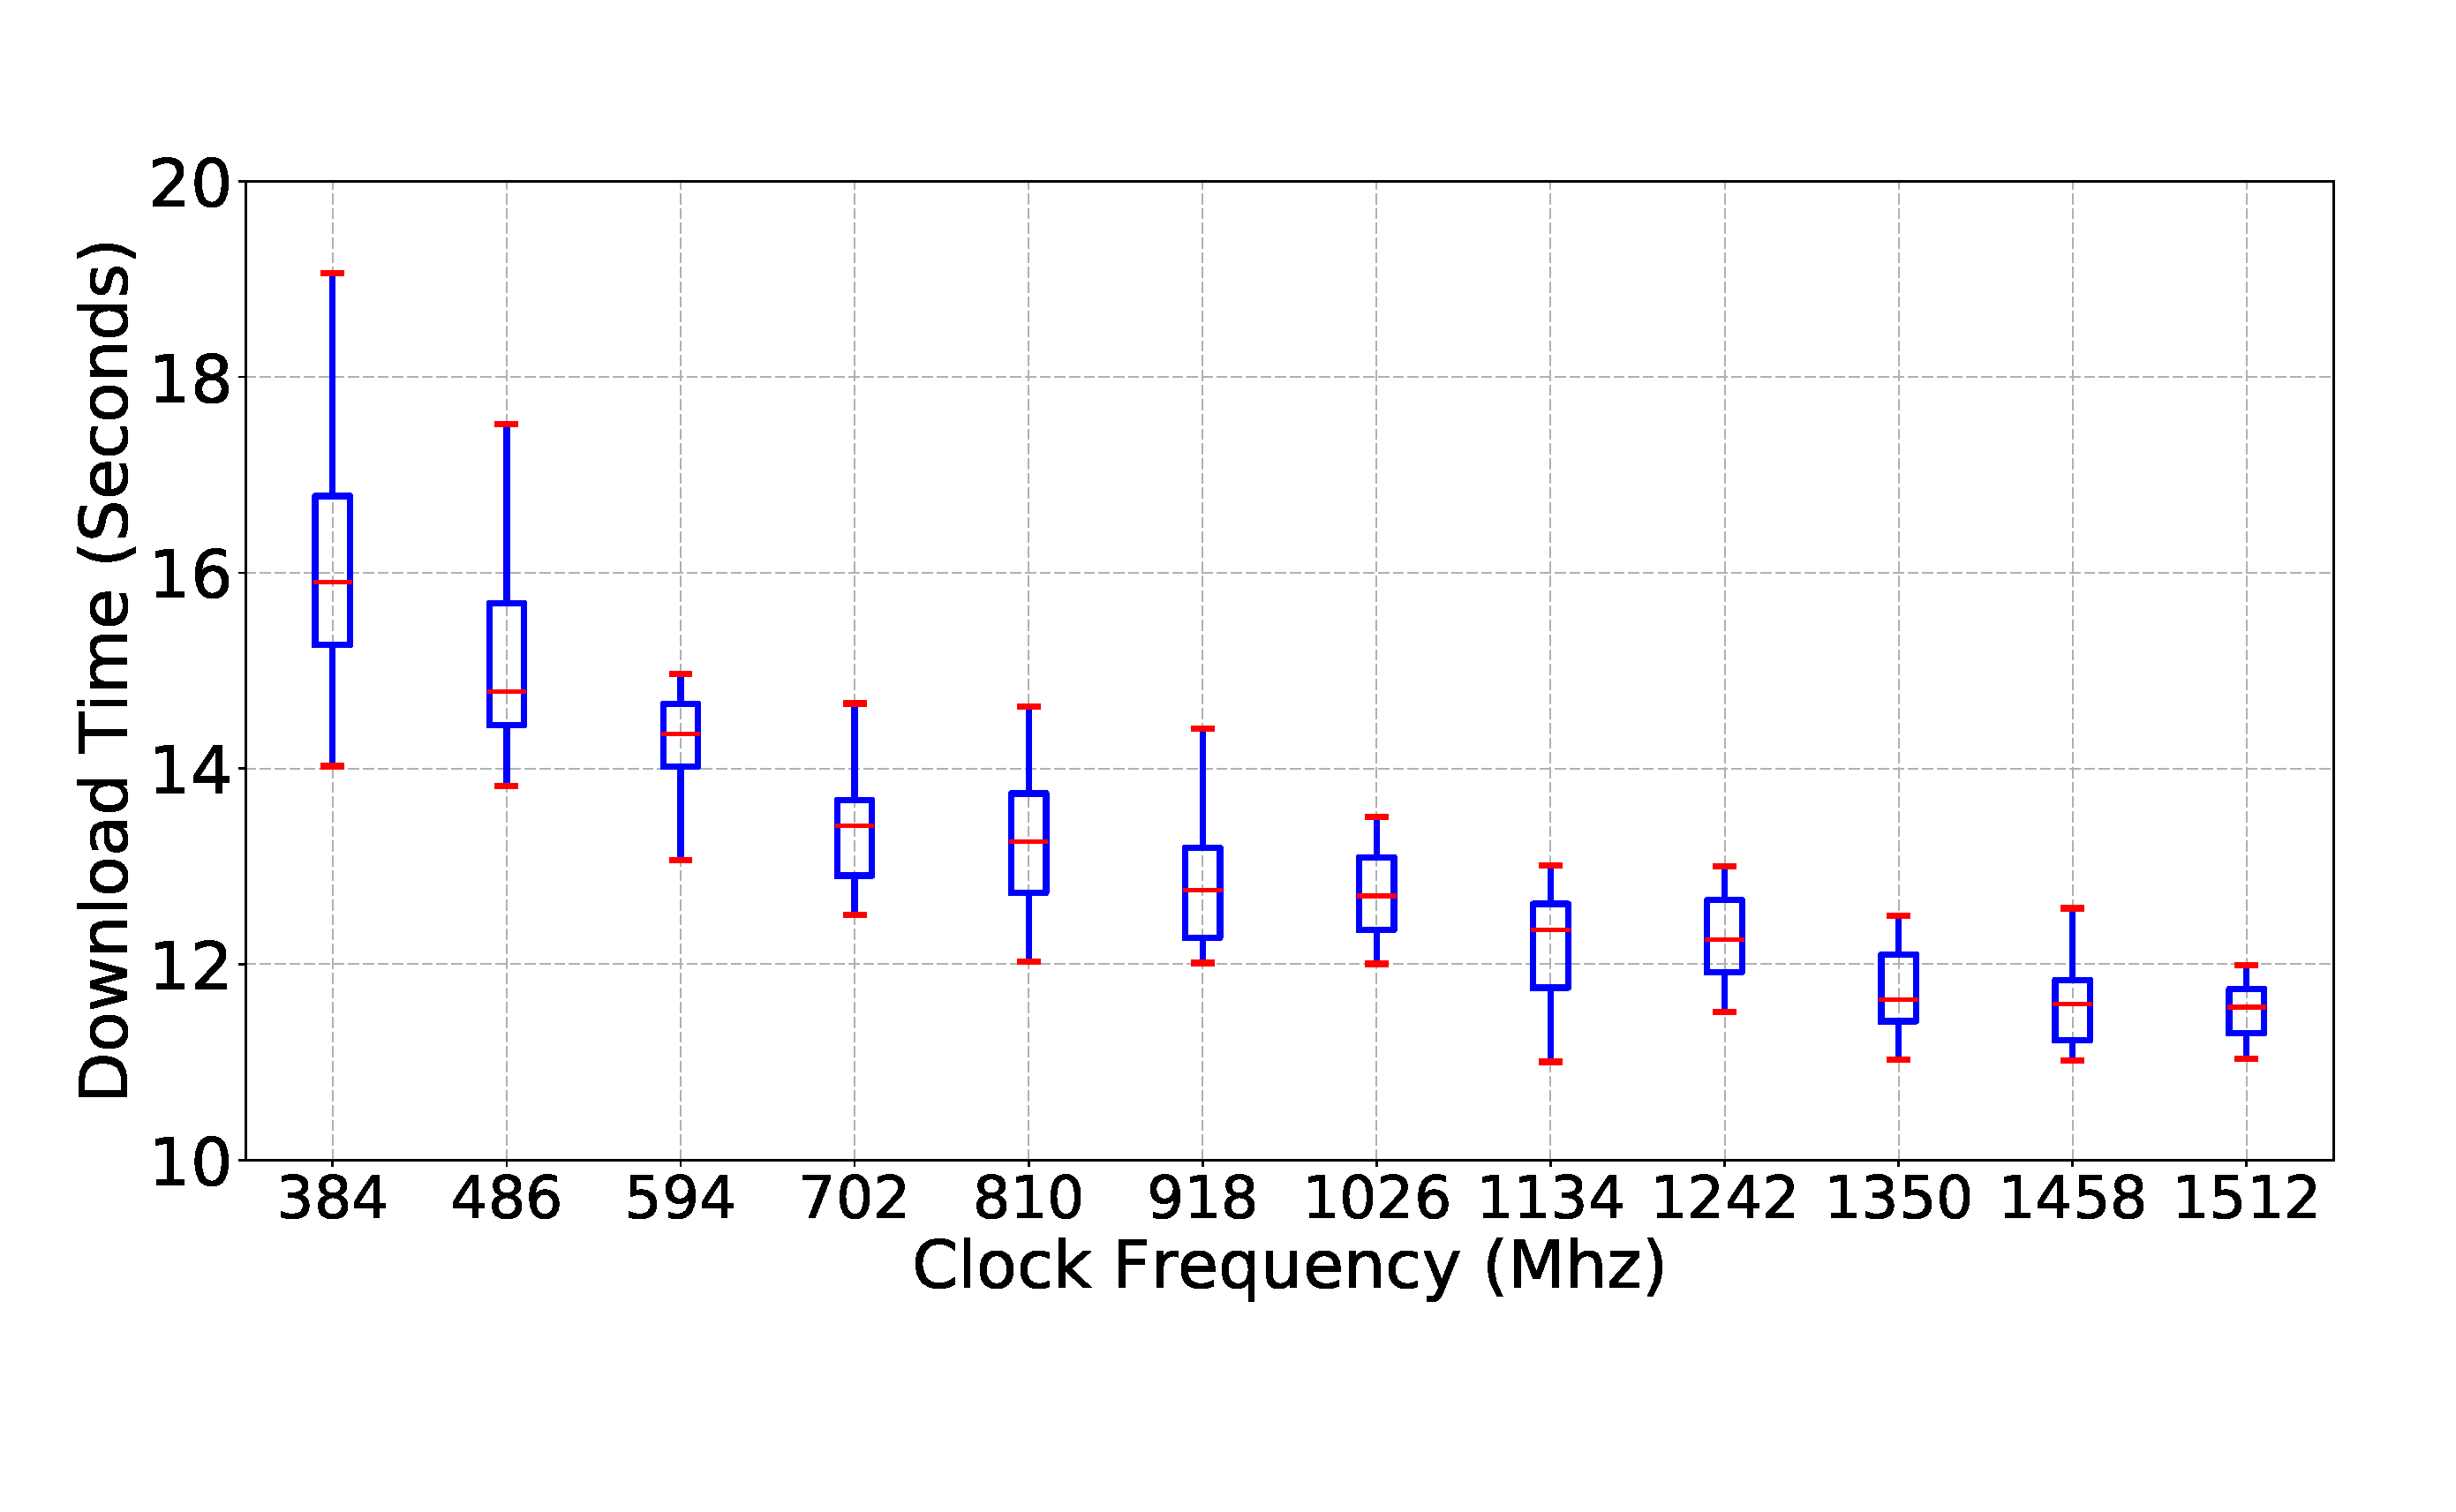
\includegraphics[width=0.5\textwidth]{sections/clock-filedownload}
     }

     \subfloat[Download Time vs. Load]{%
       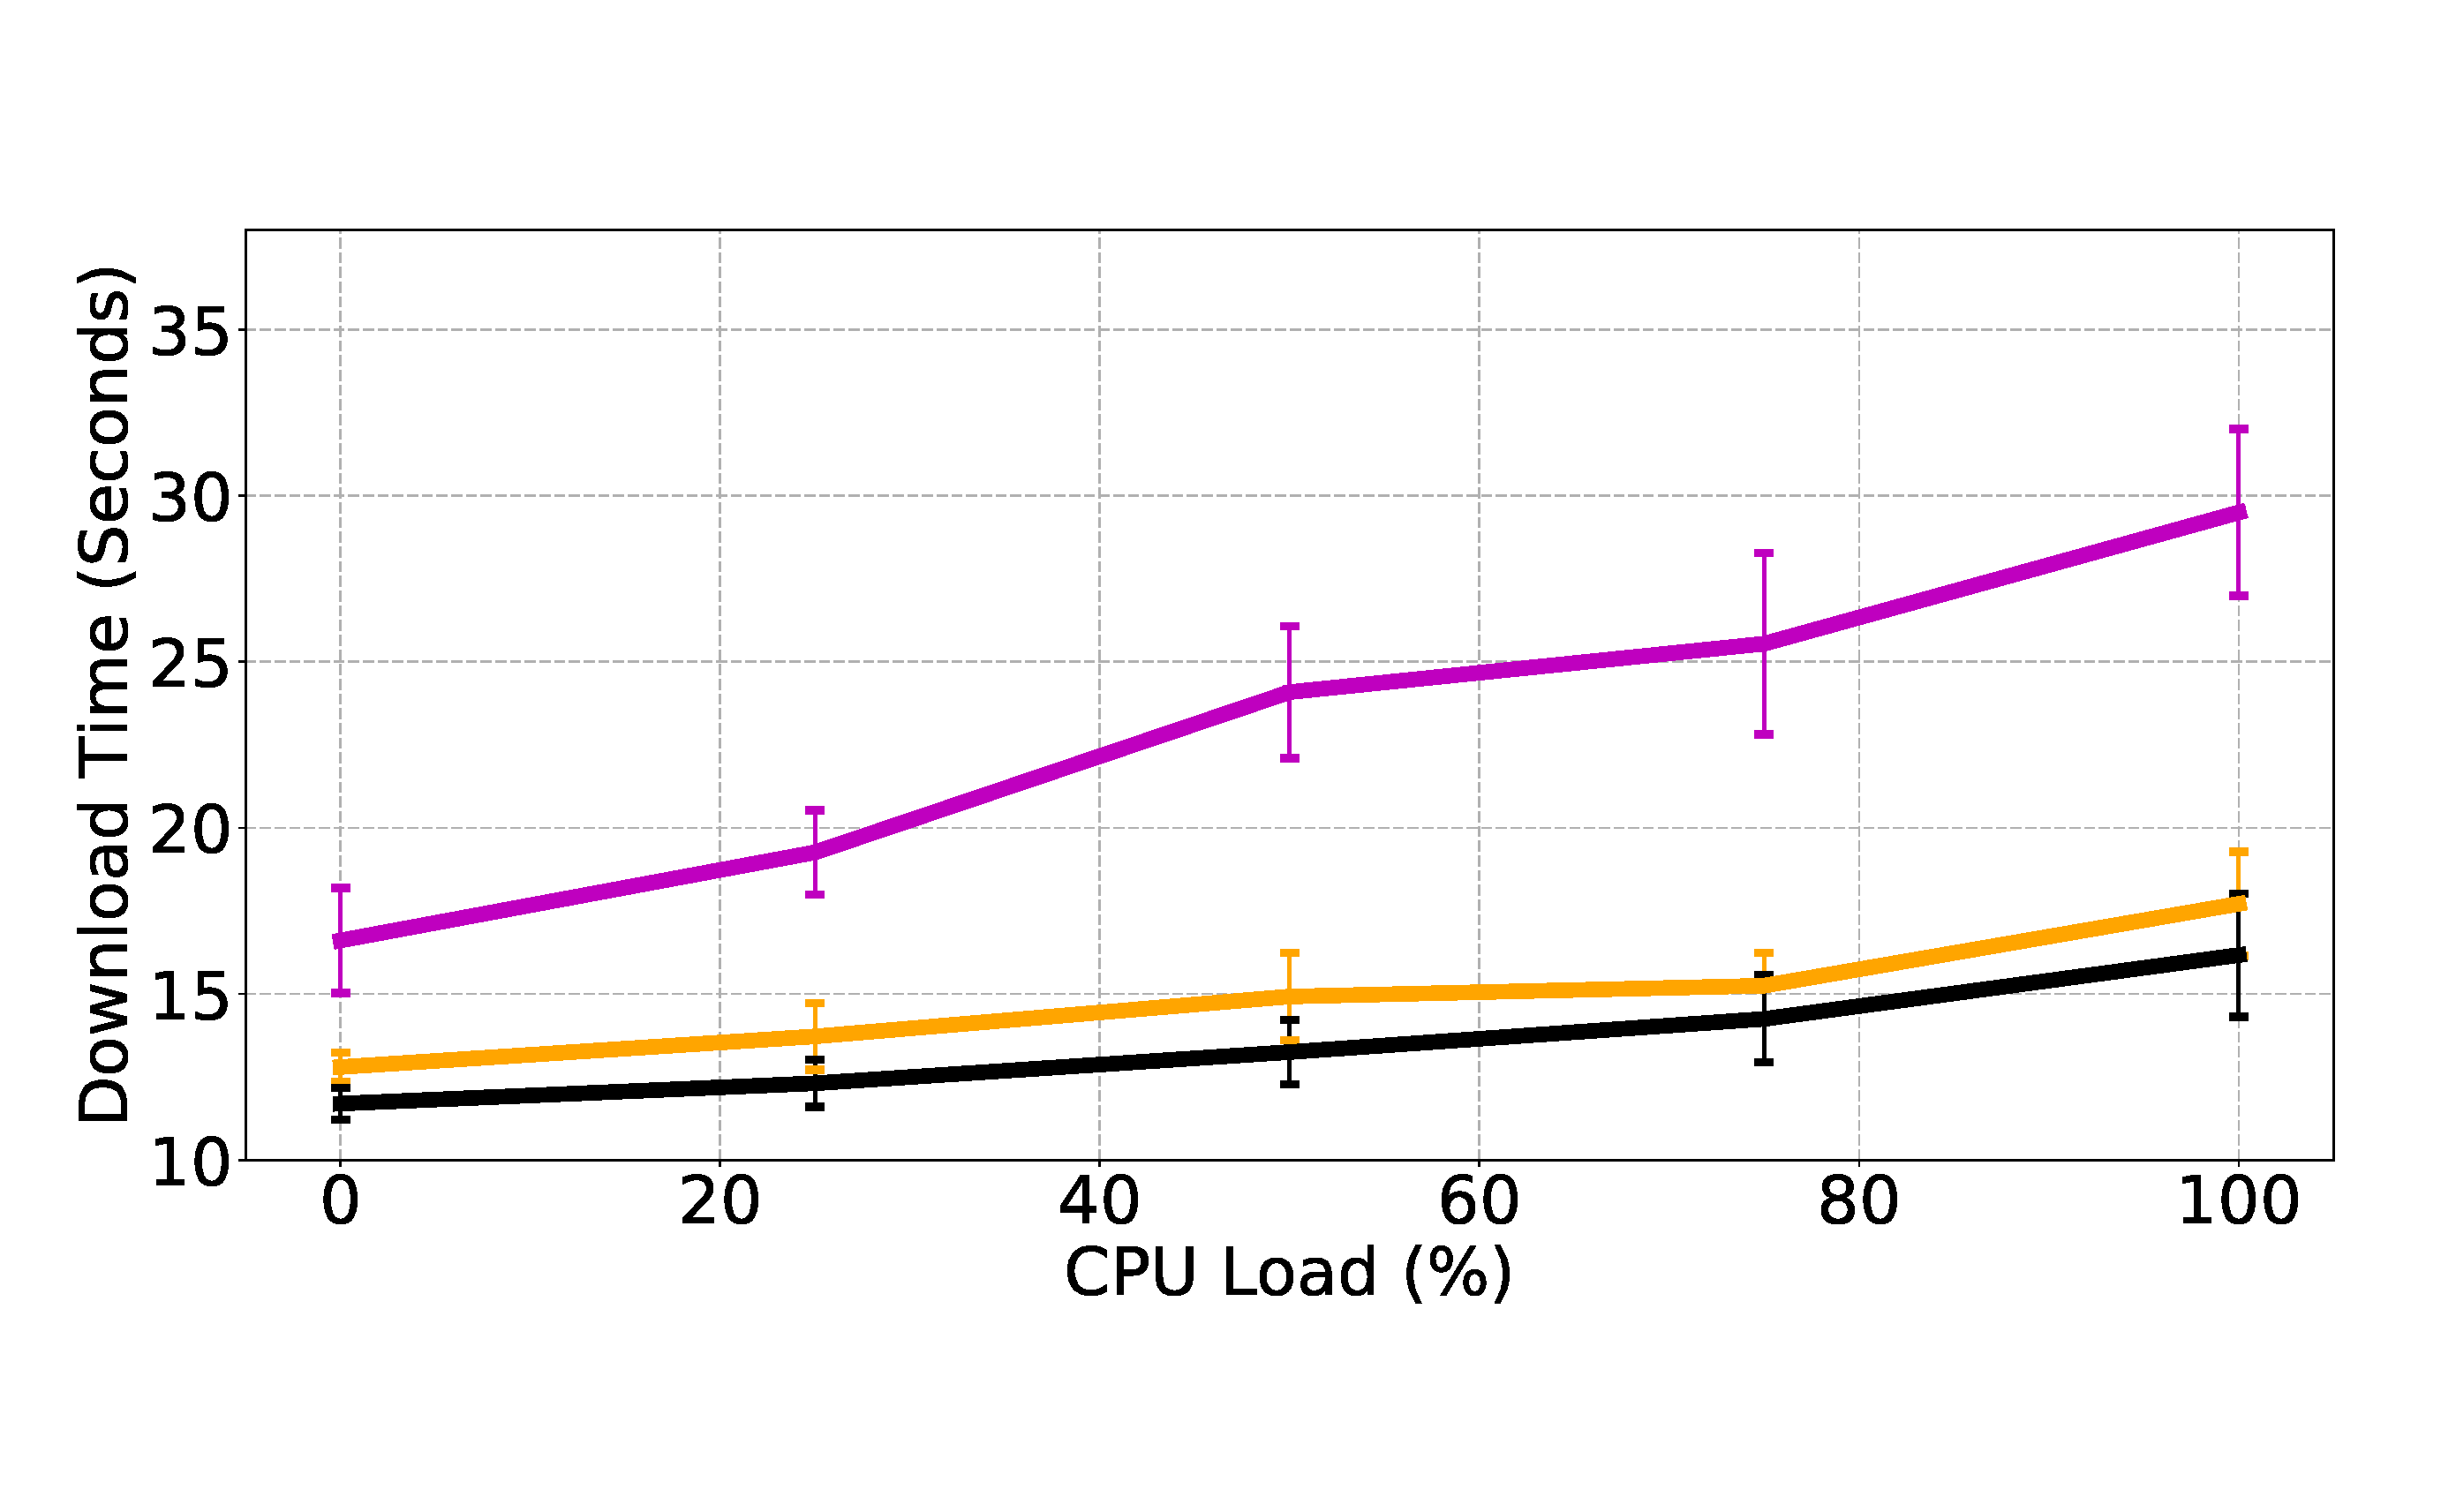
\includegraphics[width=0.5\textwidth]{sections/load-filedownload}
     }
     %\subfloat[Energy vs. Clock]{%
     %  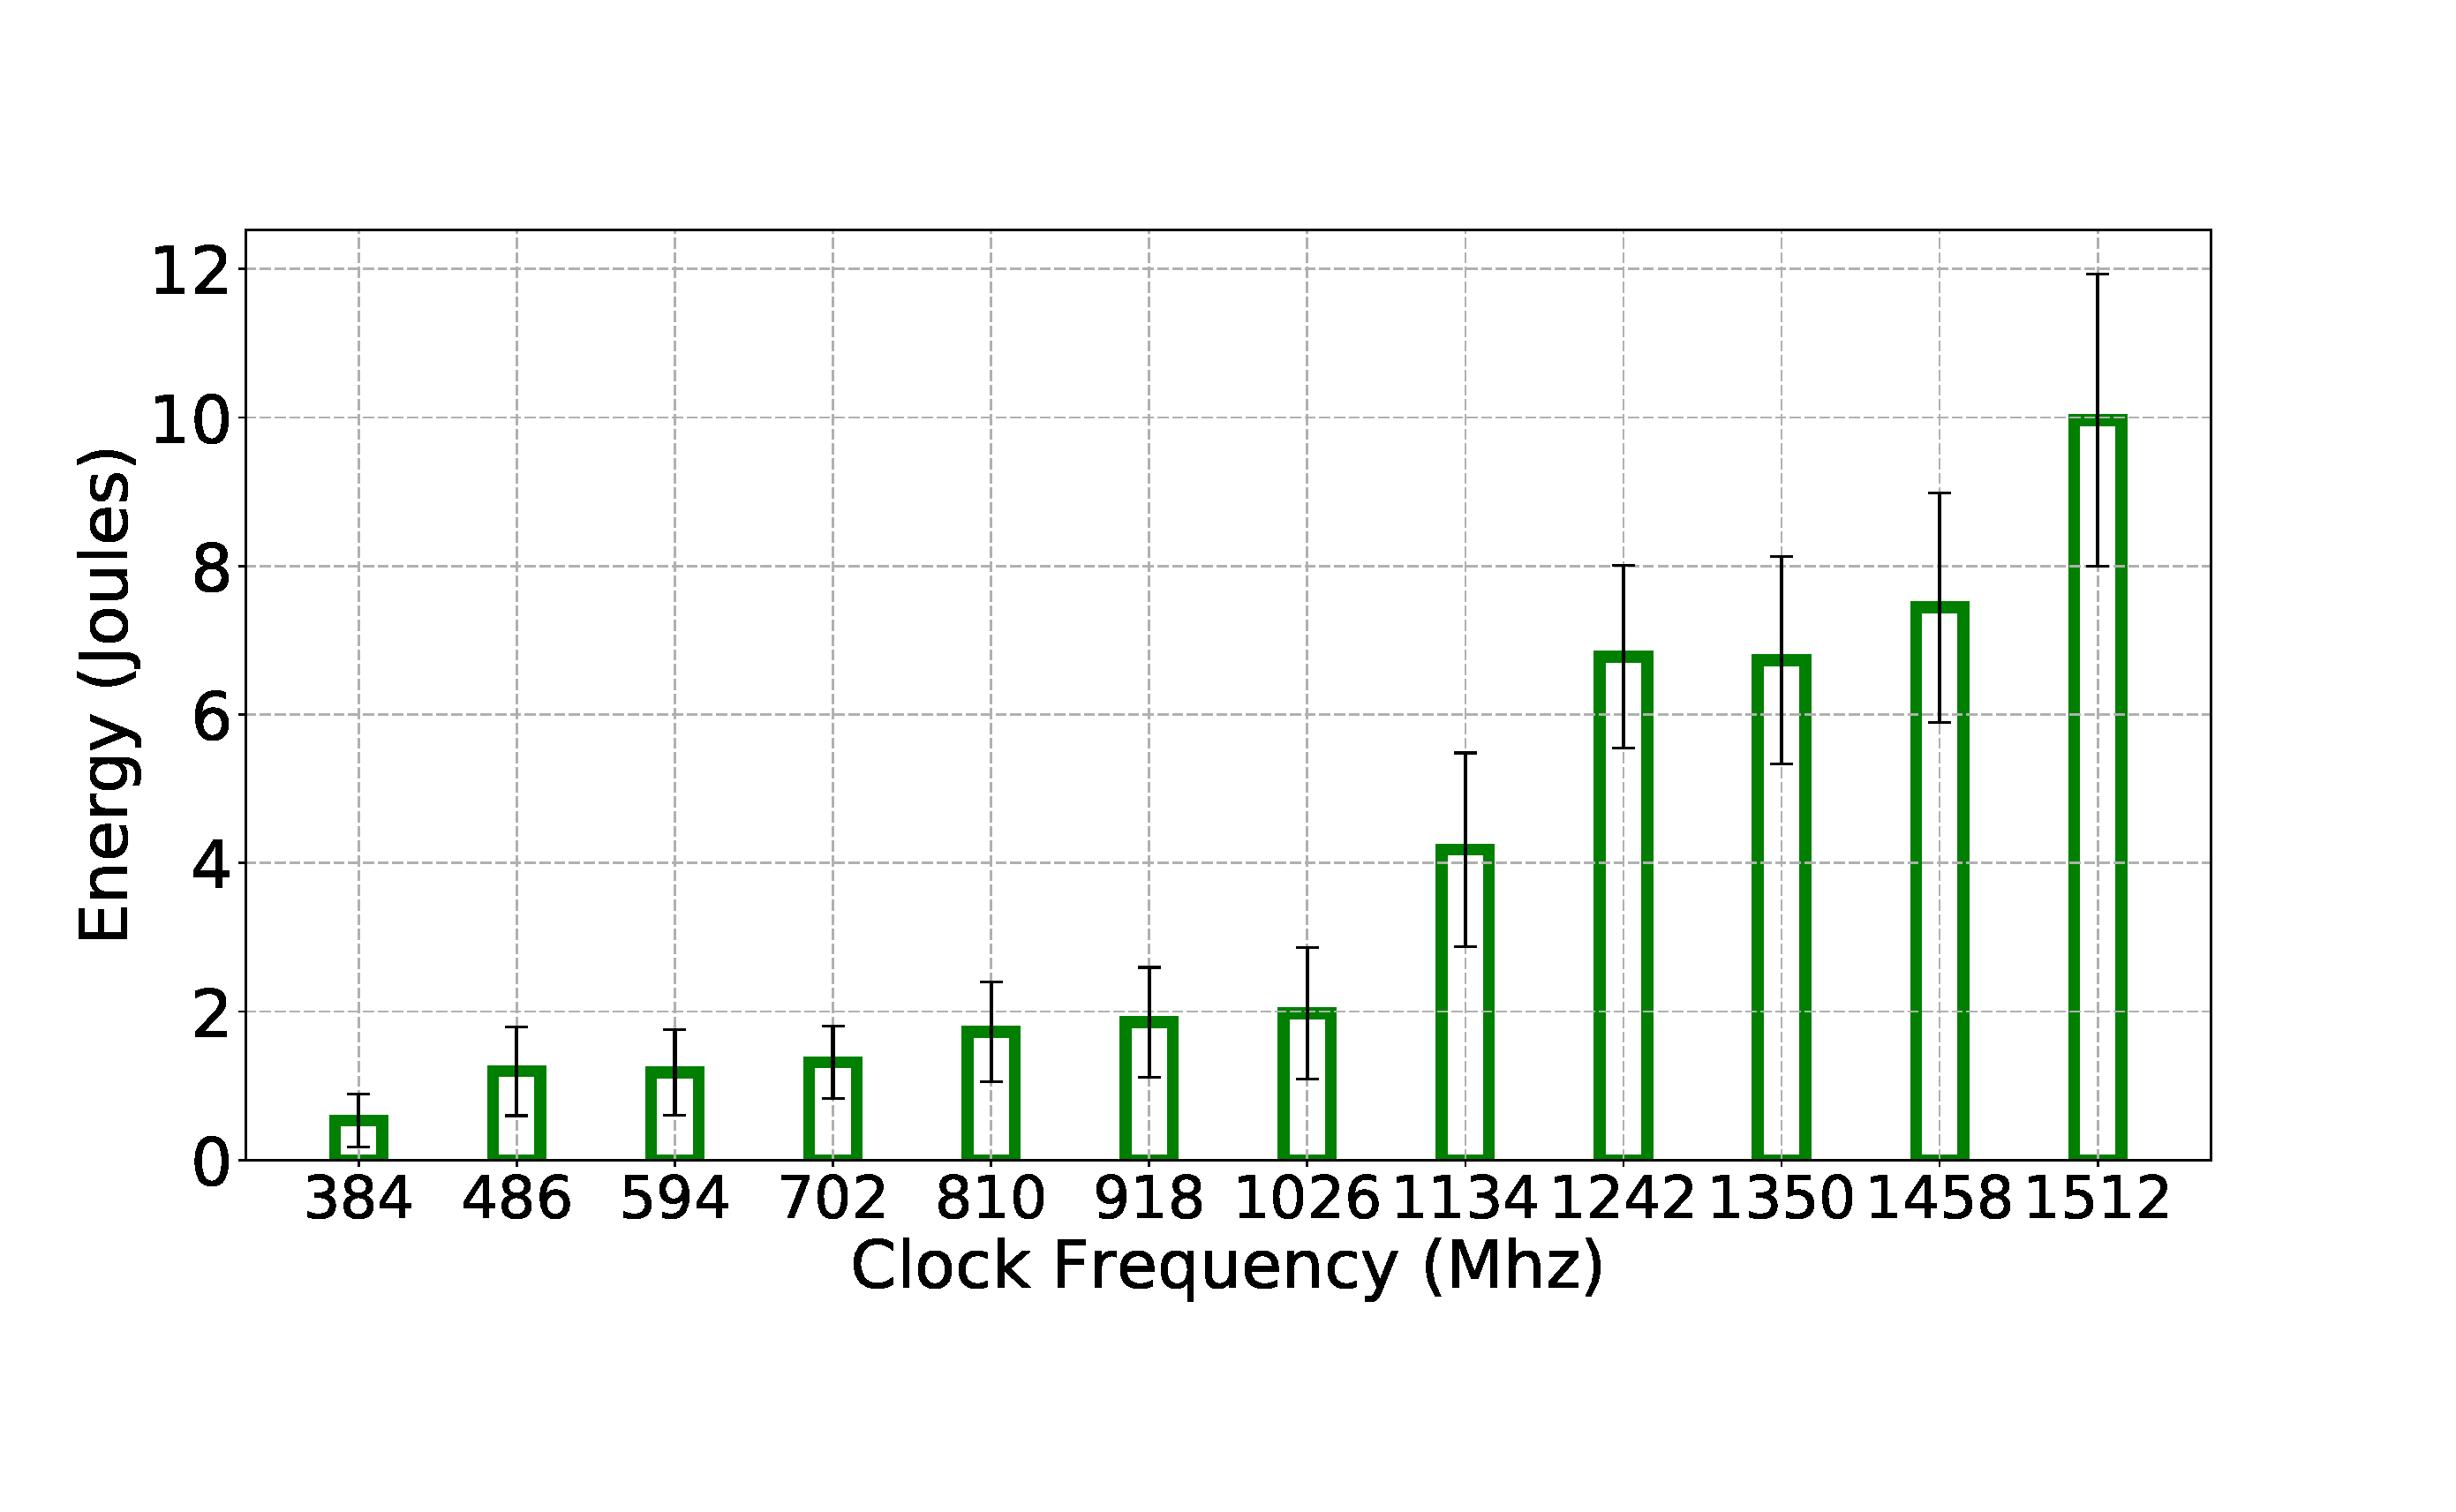
\includegraphics[width=0.34\textwidth]{sections/power-fd}
     %}
     %\vspace{-0.15in}
     %\caption{\textit{ Effect of clock frequency and load on file download: a) Linear increase from low to high clock. b) Linear increase till 50\% load then after exponential increase. c) Rapid increase in energy from 1026Mhz.}}
     \caption{\textit{ Effect of clock frequency and load on file download: a) Linear increase from low to high clock. b) Linear increase till 50\% load then after exponential increase.}}
     %\vspace{-0.25in}
     \label{fig:cycle-freq}
\end{figure}

\begin{figure}[t]
      \centering
        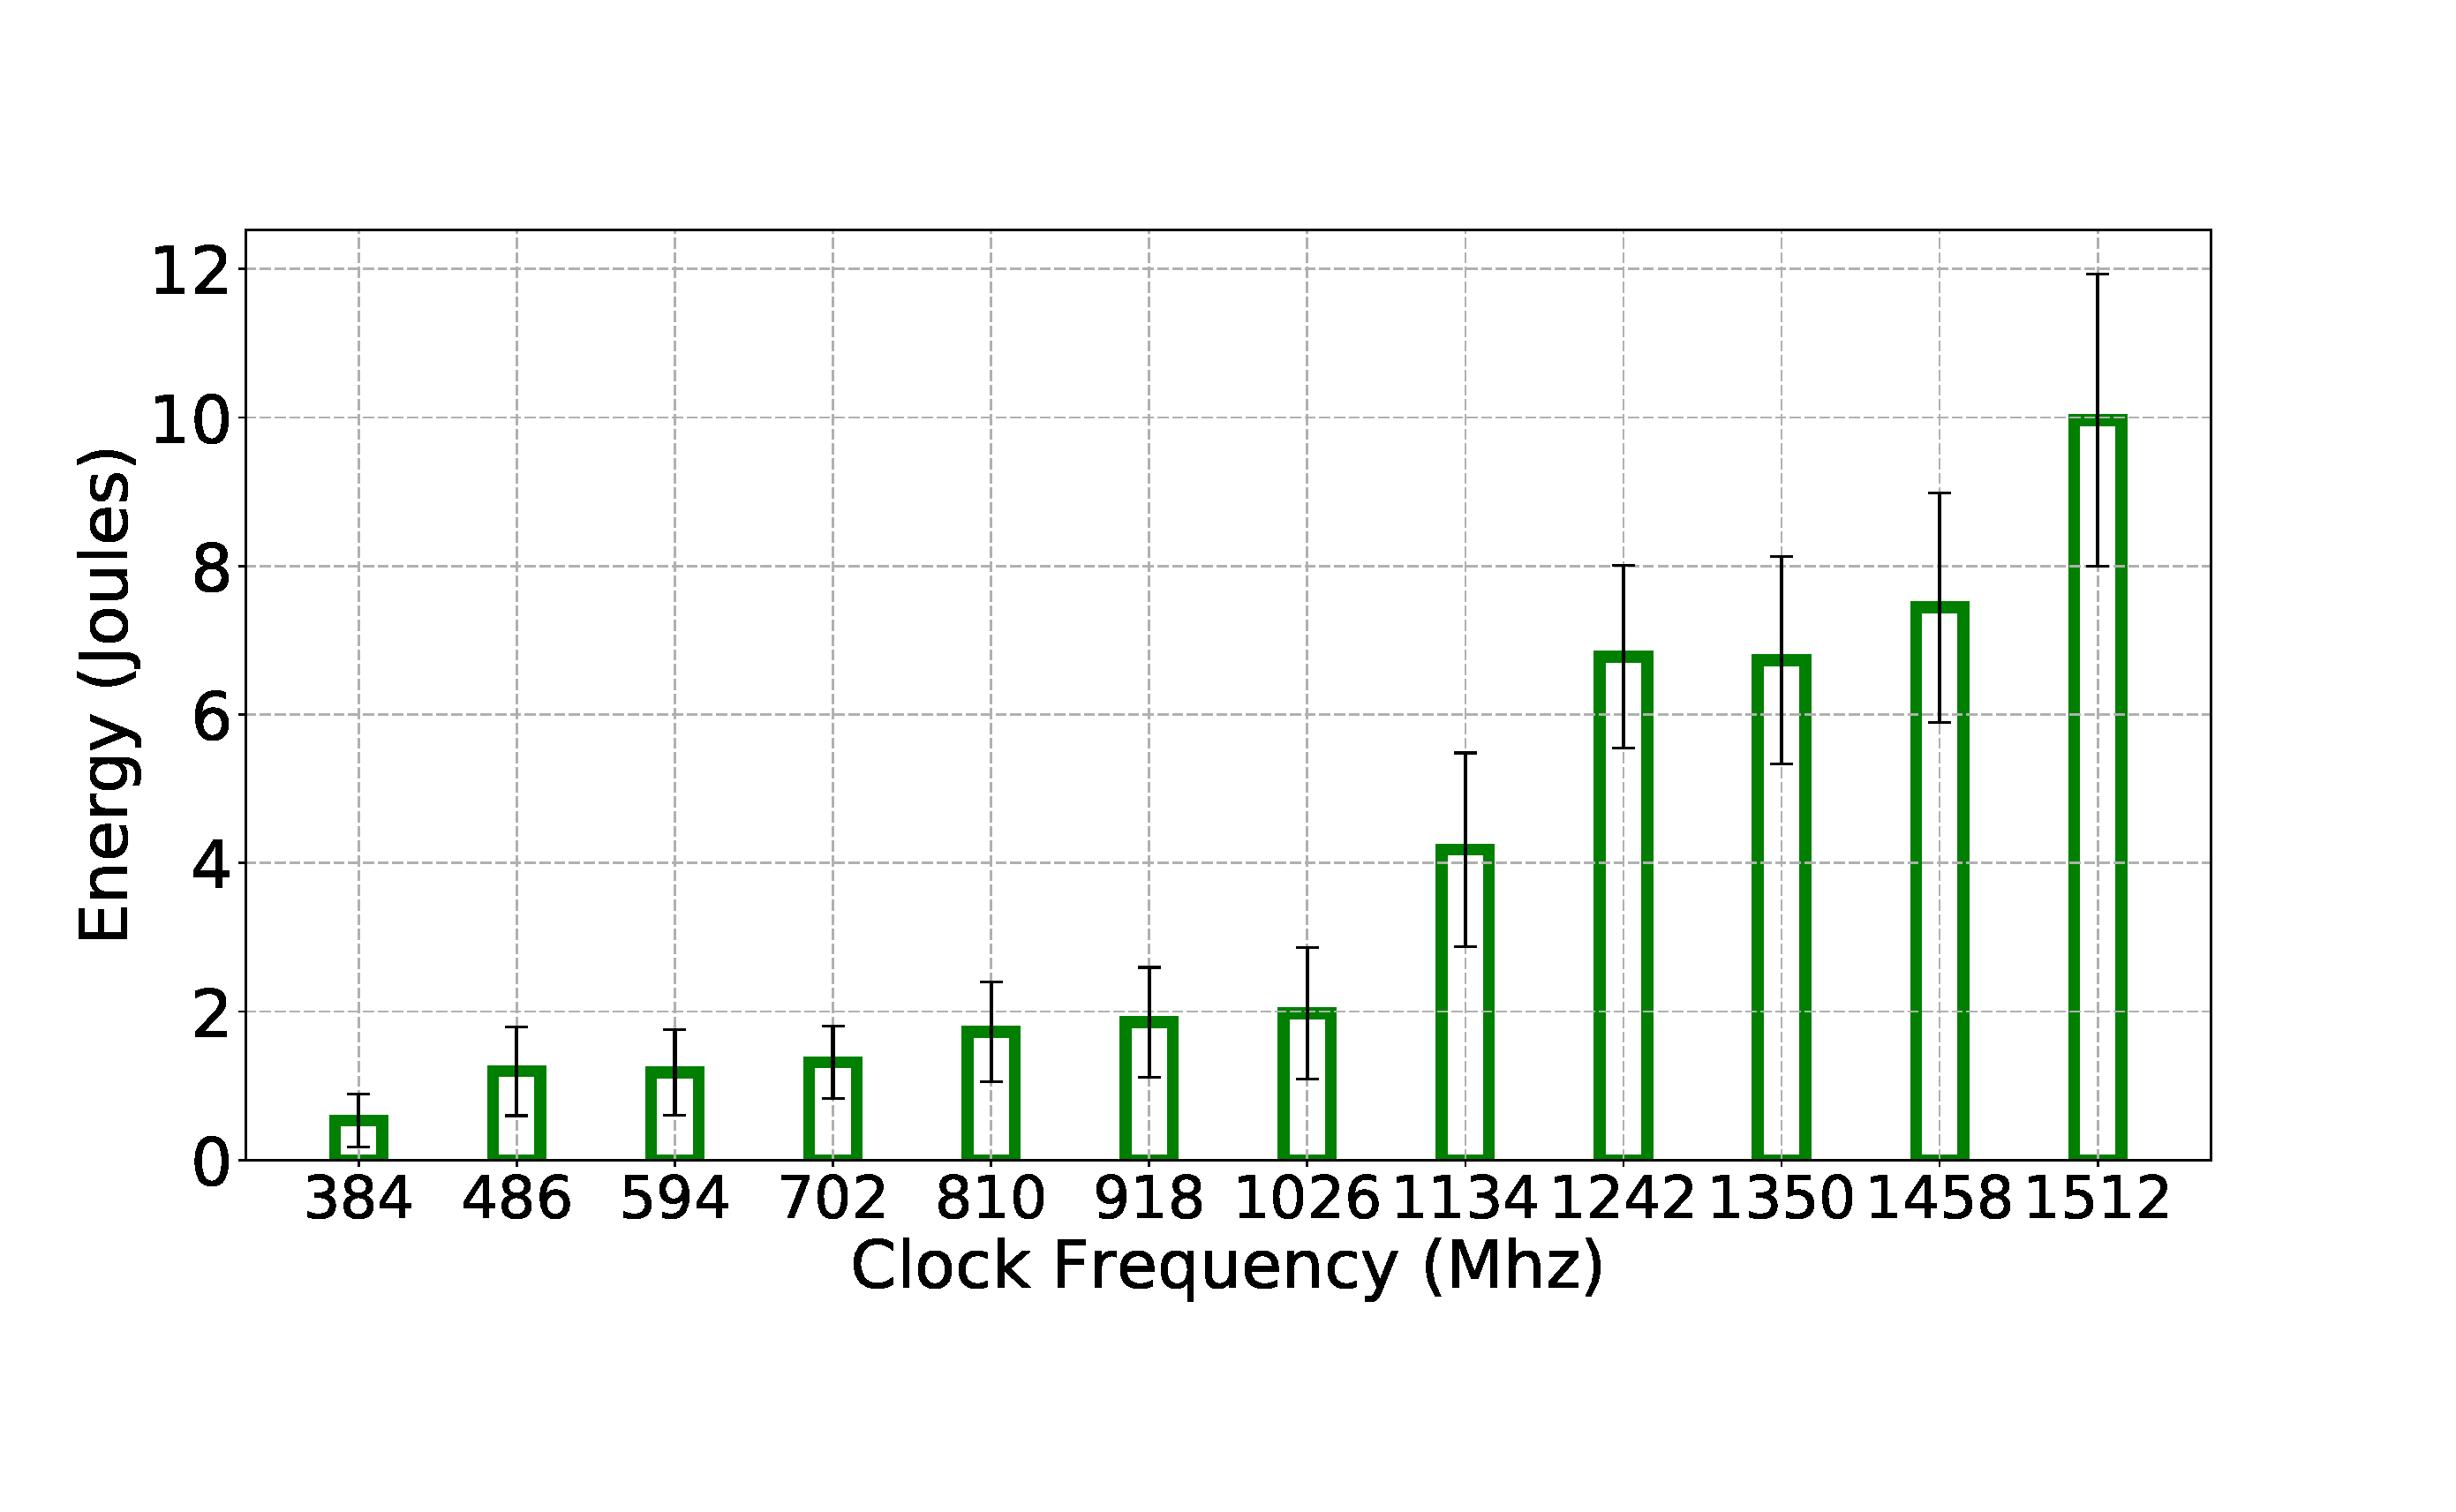
\includegraphics[width=\linewidth]{sections/power-fd}
          \caption{\textit{Energy vs. Clock during File Download. Rapid increase in energy from 1026Mhz.}}
            \label{fig:power-fd}
\end{figure}

\begin{figure}[t]
     \subfloat[Throughput vs. Clock]{%
       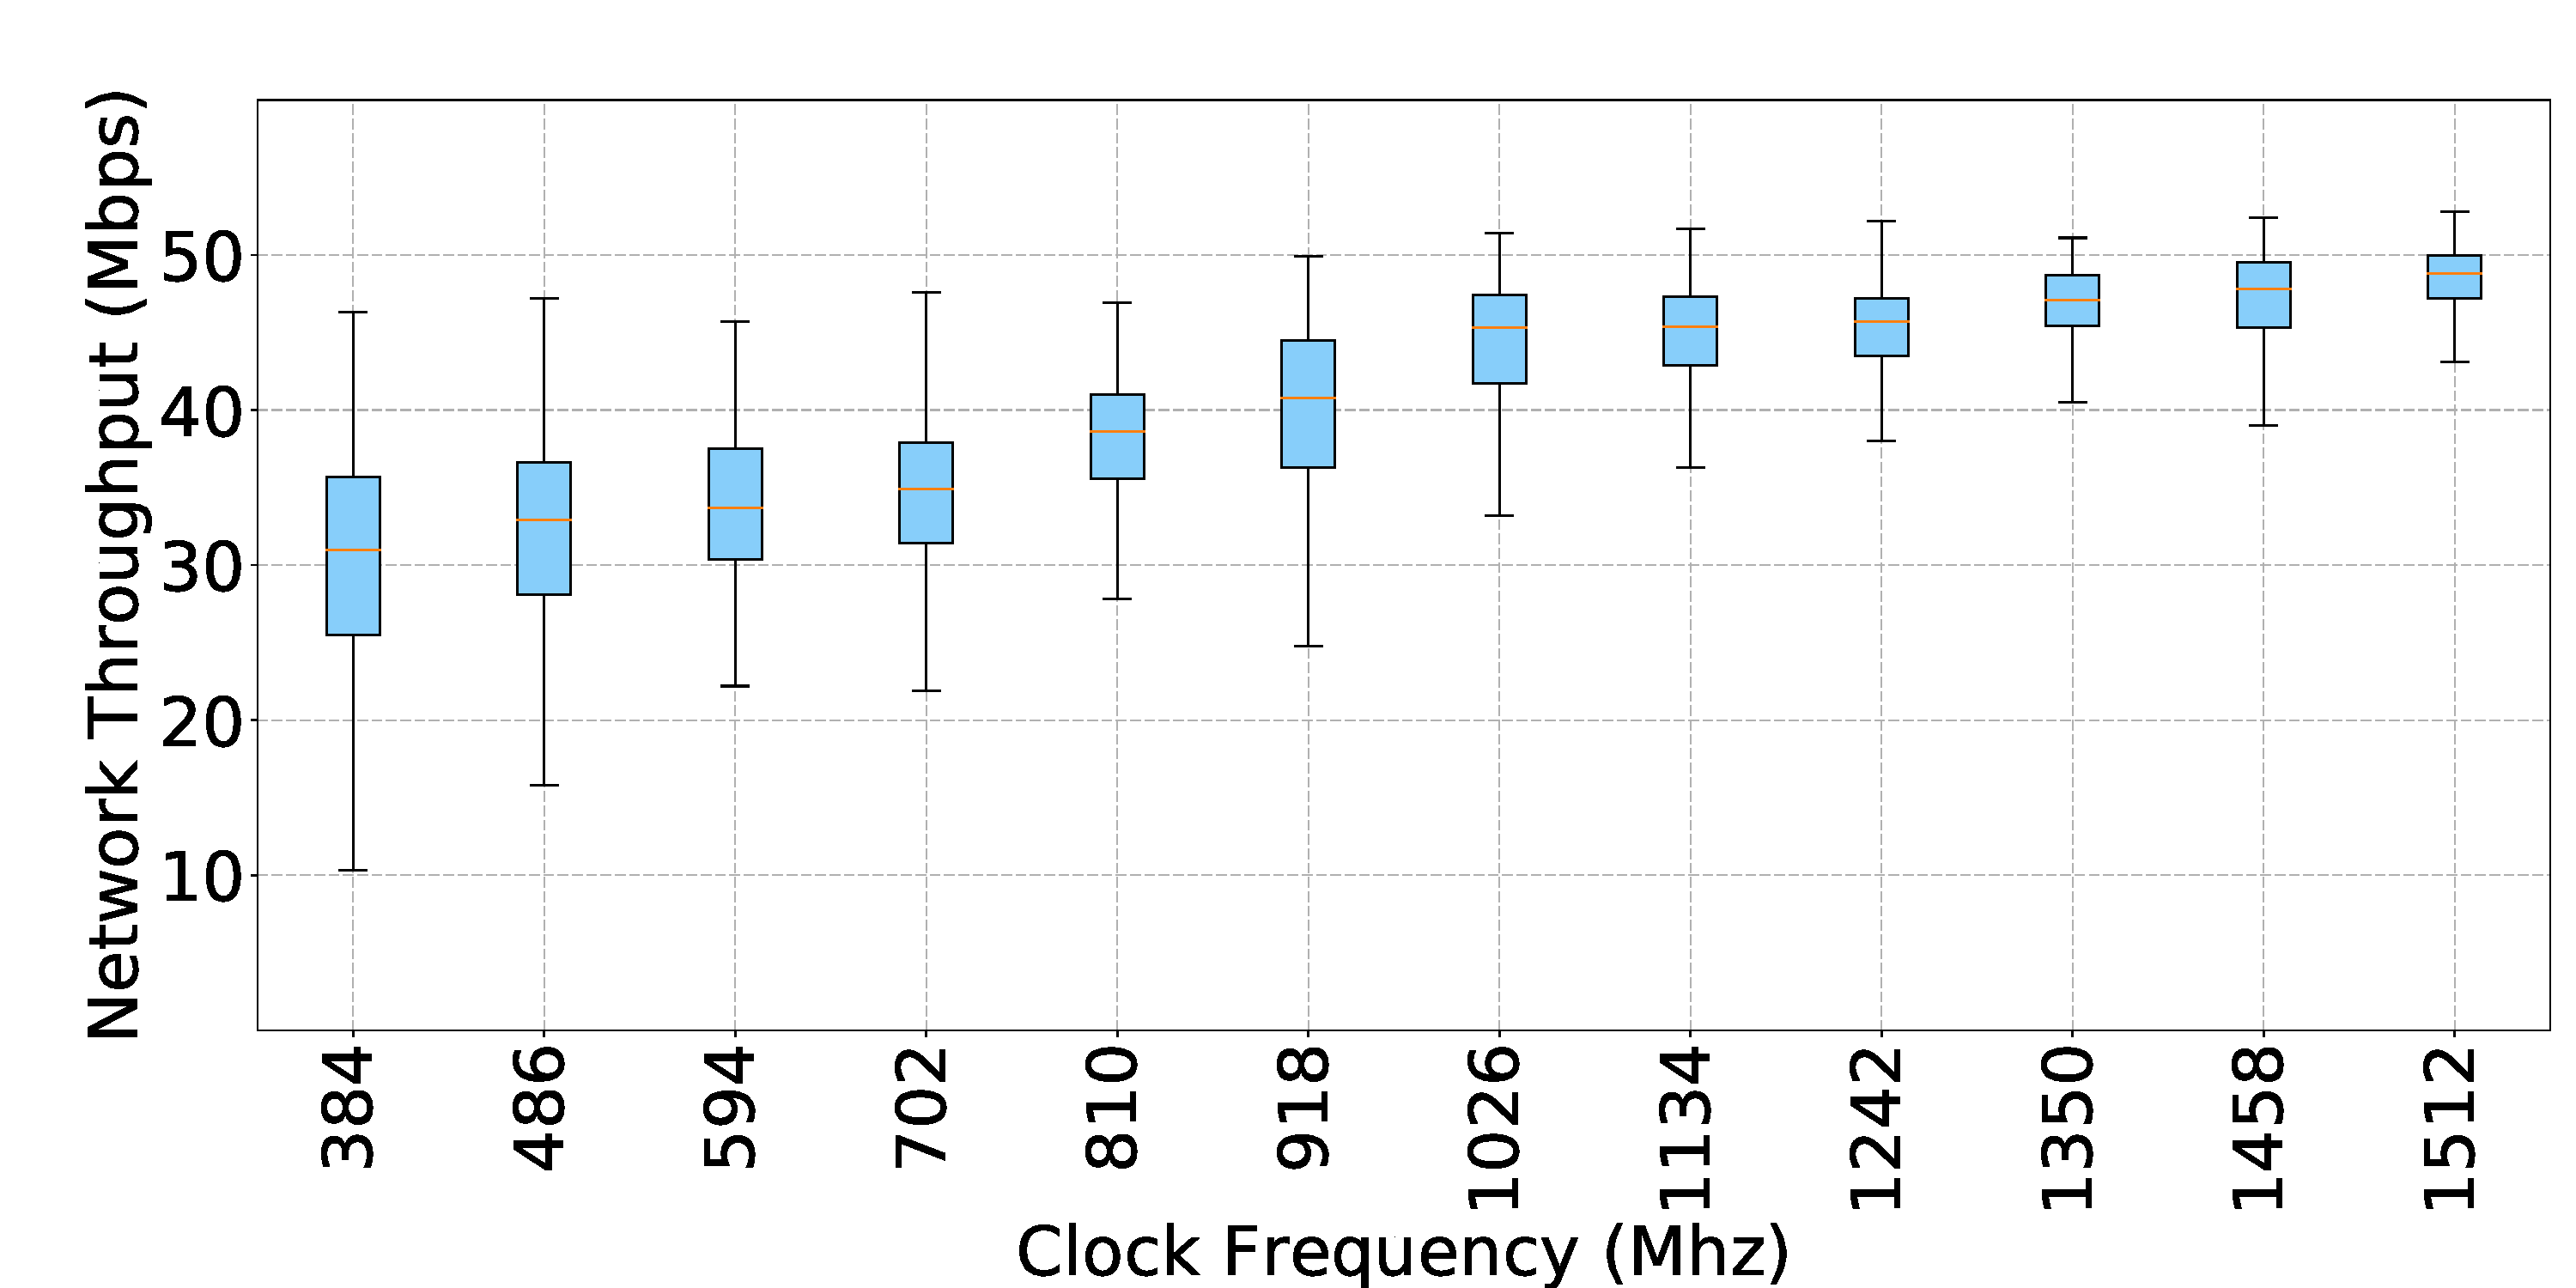
\includegraphics[width=0.45\textwidth]{sections/Throughput}
     }

     \subfloat[Throughput vs. Load]{%
       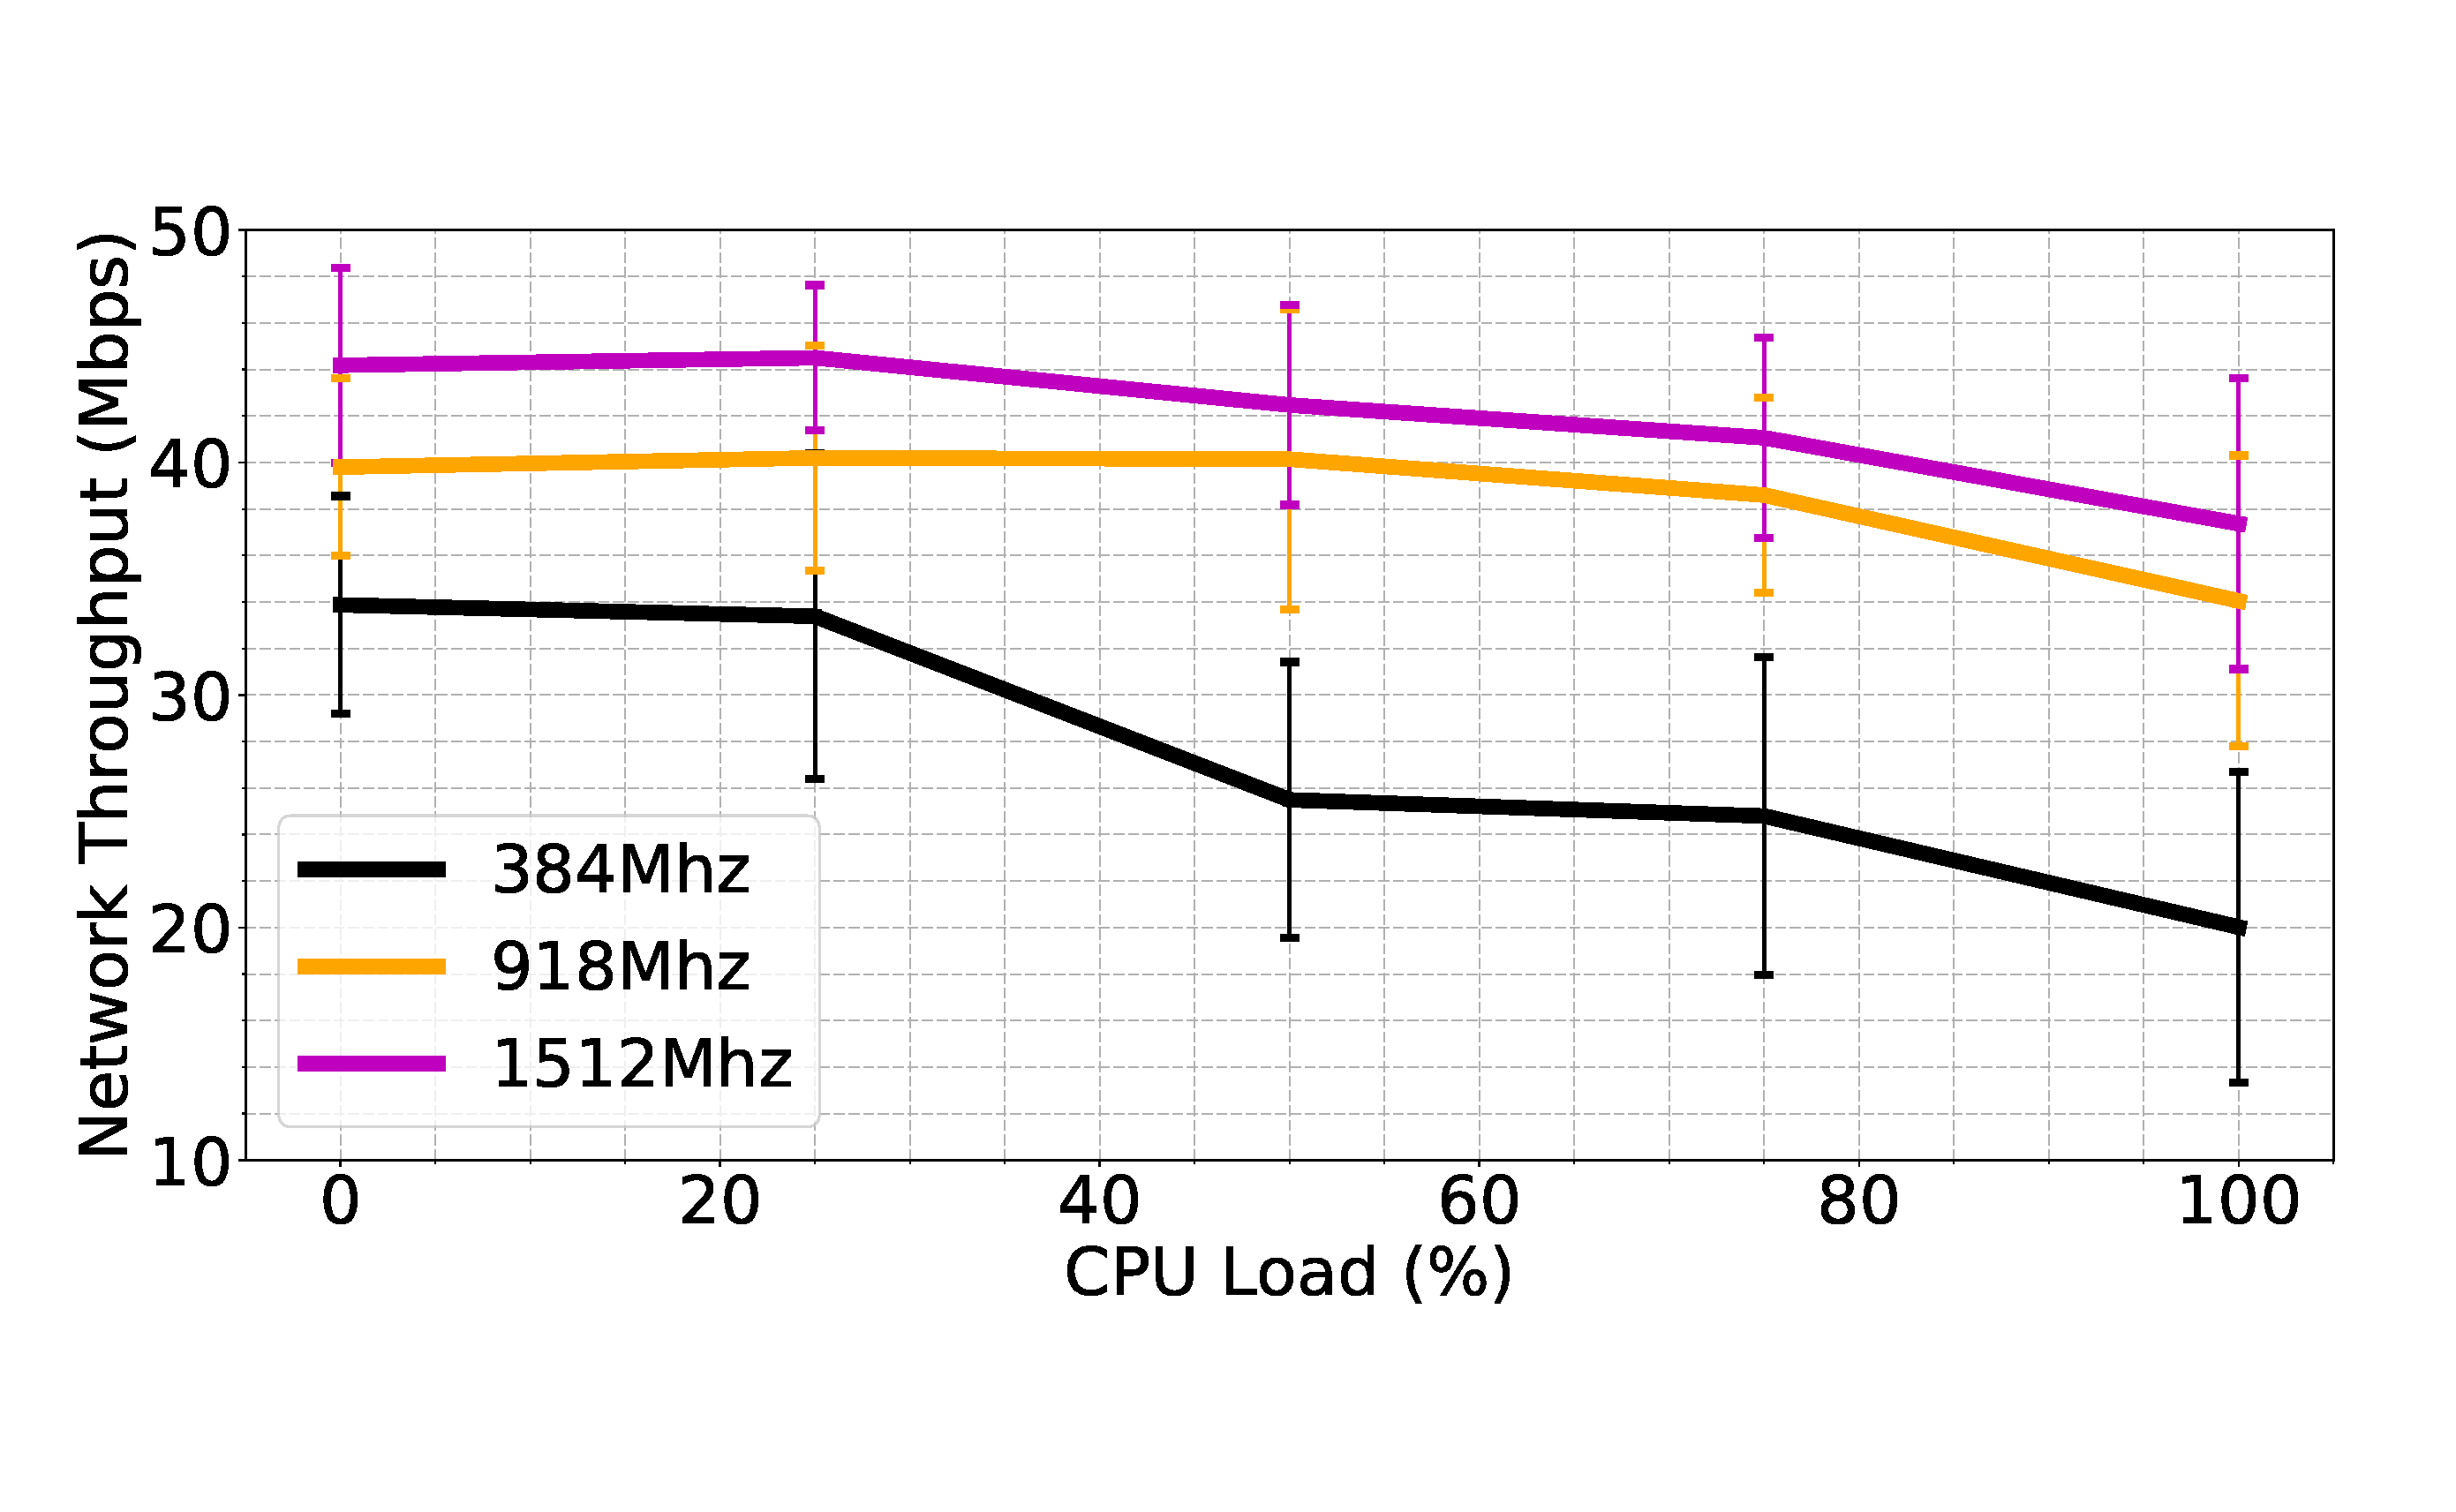
\includegraphics[width=0.45\textwidth]{sections/Load-Throughput}
     }
     %\vspace{-0.15in}
     \caption{\textit{ Effect of clock frequency and load on TCP performance: a) Linear decrease from high to low clock and high throughput variance under 384Mhz and 486Mhz clock, b) Linear decrease till 50\% load then after exponential decrease.}}
     \vspace{-0.25in}
     \label{fig:cycle-tcp}
\end{figure}
\section{File Download} \label{label:filedownload}
\textbf{Set-up}:
We use iPerf tool to measure the network throughput under controlled conditions. We host an ad hoc WiFi network using Aruba WiFi AP in an interference free environment with a link speed of 72Mbps.
We use a Linux laptop as server and Nexus4 mobile phone as a client.
We vary the CPU clock frequency and load parameters to measure both file download time and throughput.
We host a file of $50 MB$ on a server using NodeJS connected over LAN.
We load this page on the smartphone and trigger the file download automatically. Once the file download is complete, the AJAX script fires an event that calculates the total download time.
We repeat this 20 times and send the corresponding download times to our server.

Fig. \ref{fig:cycle-freq} (a) shows the download times of the file at different frequency values between $384 \ MHz$ and $1512 \ MHz$. We represent the download time in each case by the minimum, 25$^{th}$ percentile, median, 75$^{th}$ percentile and the maximum. We note that till a frequency of $702 \ MHz$, there is a sharp reduction in the download time with an increase in frequency. From $702 \ MHz$, download time reduces slowly, till it saturates at $1134 \ MHz$. We also note that the amount of variation in the download time from the median becomes smaller as the frequency increases.

Our results in Fig. \ref{fig:cycle-freq} (a) show that processing of packets is a bottleneck in the download at low frequencies, but not at higher frequencies. This shows that when only packet processing is involved, the processor can be run just at a moderate frequency of around $1134 \ MHz$.

Fig. \ref{fig:power-fd} shows the energy consumed in downloading the file at multiple frequencies. We observe that at lower frequencies, increasing the frequency value that till 1026 MHz, increasing the frequency does not affect energy consumption. Increasing the frequency further increases energy consumption rapidly. For example, at 1026 MHz, the energy consumed in downloading the file is equal to 2.3 J. This increases by over 4 times to 10 J at 1512 MHz. This is despite the fact that the download time reduces with an increase in frequency. This shows that power consumption increases at super-linear speed with an increase in clock frequency.

To check whether the CPU load affects the download time, we plot the download time of the file for different CPU loads at three frequency levels ($384 \ MHz$, $918 \ MHz$ and $1512 \ MHz$). We show the mean download times with their standard deviations in Fig. \ref{fig:cycle-freq} (b). We note that at frequencies of $918 \ MHz$ and $1512 \ MHZ$, the download time rises only by around $2 \ s$ with an increase in processor load. However, at $384 \ MHz$, the download time increases by over $13 \ s$. This shows that even applying high load on the CPU does not slow down packet processing at high frequencies.

We further plot the network throughput using Iperf for different CPU clock frequencies and CPU loads to check if they affect the performance of packet processing.
We find a similar trend in throughput trend as in the file download time.
Once again, Fig. \ref{fig:cycle-tcp} if frequency rises is below $1134 MHz$, network throughput improves with an increase in CPU frequency.
At frequencies below $1134 MHz$, the network throughput rises with an increase in the clock frequency.

This effect of hardware bottleneck on packet processing is an important issue in applications involving both high bandwidth requirements and computation.
In such cases, having poor hardware hurts performance in two different ways -- both packet processing and actual computation get slowed down.
%The network performance is severely affected by clock as shown in Fig. \ref{fig:cycle-freq} (c) and it becomes much worse when introduced load. To make it more practical, we played an HD resolution video on the mobile device while iPerf is in session, to keep some load on the device. A median difference of 20Mbps is observed from high clock to low clock. The degradation is largely due to the high throughput variance in the case of low clock. This variance drastically reduced under higher clock frequencies. We observed a little less (<15Mbps) change when there is no such artificial load on the device. To quantify the impact of load on network performance, we created artificial CPU load and tested under three clock frequencies. The load is affecting the performance severely in the case of low clock and nominally under high clock. The worst case median throughput difference under 100\% load under low clock and no load under high clock is > 20Mbps. 

%This shows a triangle-effect of hardware bottlenecks on web performance: A direct effect of these hardware parameters on web performance and a direct effect on network performance that could indirectly affects the web performance in downloading of web objects.
